\MTtitle{Aplicación Web}

%--------------------------------------Internet--------------------------------------------%


\section{Aplicación Web}
Las aplicaciones Web permiten la generación automática de contenido, la creación de páginas personalizadas según el perfil de usuario o el desarrollo de comercio electrónico.

\section{Patrón de diseño}
Para el análisis y desarrollo de aplicaciones es necesario seguir una técnica para tener el control de la aplicación, con el fin de darle mantenimiento. Se han desarrollado múltiples técnicas que cumplen con esta tarea.\\


El patrón deseable para el desarrollo de aplicaciones Web es el Modelo Vista Controlador (MVC), este modelo considera separar en tres capas un proyecto, permitiendo gestionar sistemas de software grandes y complejos, el cual puede ser implementado en sistemas Web.

\begin{itemize}
	\item Lógica de control: saber qué elementos tiene el proyecto y qué hacer, pero no cómo se implementó
	\item Lógica de negocio: saber cómo se desarrolla la aplicación
	\item Lógica de presentación: saber cómo interactúa el usuario con la aplicación
\end{itemize}
El patrón Modelo Vista Controlador, es el más extendido para el desarrollo de aplicaciones donde se deben manejar interfaces de usuarios, éste se centra en la separación de los datos o modelo, y la vista, mientras que el controlador es el encargado de relacionar a estos dos.
\\
La Figura \ref{fig:modVisCont} muestra la separación de las tres capas.
\begin{figure}[H]
  \centering
  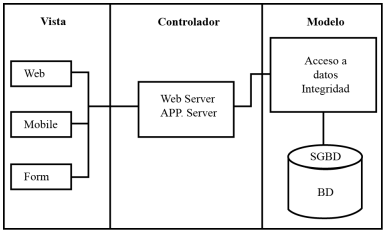
\includegraphics[scale=.50]{imagenes/Capitulo3/mvc.png}
  \caption{Patrón MVC Modelo Vista Controlador.}
  \label{fig:modVisCont}
\end{figure}

\section{Framework}
Un marco de trabajo (\textit{Framework}) es una colección integrada de componentes, la cual simplifica el desarrollo de aplicaciones, al proporcionar bibliotecas y herramientas de software.\\


JavaServer Faces (JSF) es un Framework para aplicaciones Web que simplifica el diseño de la interfaz de usuario y separa aún más la presentación de una aplicación Web de su lógica comercial.
\\
JavaServer Faces proporciona dos bibliotecas de etiquetas personalizadas para agregar los componentes a una página. El programador diseña la apariencia visual de una página con JSF, agregando etiquetas

\section{Internet}

Son muchas las definiciones que se encuentran de la Internet, sin embargo su definición es simple, 
''la Internet es una colección de redes de comunicación interconectadas mediante el protocolos 
lo cual lo cual garantiza que las redes físicas que la componen, formen una red lógica única de 
alcance mundial'' \citep{CTInternet}.
\\

Uno de los principales objetivos cuando se desarrolló fue permitir la comunicación entre distintos usuarios,
hoy en día es utilizado para muchos ámbitos, desde obtener información relevante, hasta comprar artículos 
provenientes de otros países.
\\

El Instituto Nacional de Estadística y Geografía (INEGI) realizó una encuesta\footnote{https://www.inegi.org.mx/programas/dutih/2018/}  
en donde se muestra que al año 2018 hay 18.3 millones de hogares que disponen de Internet, es decir más del 
50\% de la población en México.
El acceso a Internet ha crecido de manera exponencial, permitiendo a los usuarios tener infresar a distintos recursos.

%se puede enviar y reciibir información al mismo tiempo y a través de las mismas rutas de comunicación.

%------------------------------------World Wide Web--------------------------------------------%

\subsection{World Wide Web}

La WWW \textit{World Wide Web} es un sistema de distribución de documentos HTML \textit{HyperText Markup Language} 
que permite a los usuarios de computadora ejecutar aplicaciones basadas en Web, además de localizar y ver documentos 
basados en multimedia sobre casi cualquier tema a través de Internet.
La \textit{World Wide Web} es una colección gigante de documentos o páginas, almacenados en computadoras de todo el mundo. 
Comúnmente llamada la Web, esta colección de páginas representa una gran cantidad de texto, imágenes, audio y video disponibles 
para cualquier persona con una computadora y una conexión a Internet.

%--------------------------------------HTML-------------------------------------------%
\Tlabel{cp3:html}
\section[HTML]{Hypertext markup language}
HyperText Markup Language (\textit{HTML}, por sus siglas en ingles), 
es un lenguaje que permite presentar contenido en la Web y fue propuesto por primera vez por 
Tim Berners-Lee (1989). El estándar ha evolucinado continuamente desde su introducción inicial, 
la versión más reciente es HTML5 que está siendo desarrollada por el \textit{World Wide Web Consurtium} (W3C).
\\
Un archivo HTML es un texto sin formato, el cual se puede abrir y editar con cualquier editor de 
texto. Lo que hace al HTML tan poderoso es su estructura marcada, el cual permite definir las partes 
de un documento que deben mostrarse como titulares, las partes que contienen enlaces, las partes que deben 
organizarse como tablas y muchas otras formas. Las definiciones de marcado se basan en secuencias de caracteres 
predefinidas, las etiquetas, que encierran partes del texto \citep{CTHTML}. 

%--------------------------------------Sitios Web------------------------------------------%

\section{Sitios Web}
Un sitio Web es un conjunto de páginas Web relacionadas entre sí. Se entiende por página Web tanto el fichero 
que contiene el código HTML como todos los recursos que se emplean en la página, como pueden ser
imágenes sonidos, videos \citep{CTsW}.
Un sitio Web son de acceso público que comparten un solo nombre de dominio, pueden ser creados y 
mantenidos por un individuo, grupo, empresa u organización para cumplir una variedad de propósitos. 
Todos estos sitios constituyen la World Wide Web. 

%---------------------------------------Página Web------------------------------------------%

\subsection{Página Web}

Una página Web es un documento electrónico el cual forma parte de la WWW (\textit{World Wide Web}) generalmente 
construido en el lenguaje HTML (\textit{Hyper Text Markup Language}). Este documento puede contener enlaces que nos 
direcciona a otra página Web. Para visualizar una página Web es necesario de un browser o un navegador. 
Dentro de las páginas Web se encuentra un sinfin de sitios los cuales pueden ser de interés. 
Las páginas Web pueden ser estáticas o dinámicas. Las páginas estáticas muestran el mismo contenido cada vez que se 
visualizan. Las páginas dinámicas tienen contenido que puede cambiar cada vez que se accede a ellas \citep{CTpW}. 

%-------------------------------------------Blog------------------------------------------%

\subsection{Blog}

Un blog es una página Web en la cual el usuario no necesita conocimientos específicos del medio electrónico ni del 
formato digital para poder aportar contenidos de forma inmediata, ágil y constante desde cualquier punto de conexión 
a Internet \citep{CT17}. \\
Un blog es un sitio Web que generalmente contiene información realizada por un autor. Esta información pueden ser de varios 
tipos, como comentarios, descripciones de eventos, fotos, videos, comentarios personales, tutoriales, estudios de casos, artículos 
de opinión extensos, ideas políticas o cualquier otra cosa que pueda imaginar. Por lo general, se muestran en orden cronológico 
inverso, con las adiciones más recientes en la parte superior. Esas entradas de información se pueden organizar de varias maneras, por fecha, tema. 
Una de las características principales de un blog es que se debe actualizar periódicamente. A diferencia de un sitio Web donde el 
contenido es estático, un blog se comporta más como un diario en línea, donde el blogger publica actualizaciones periódicas. Por lo 
tanto, los blogs son dinámicos con contenido siempre cambiante. Un blog se puede actualizar con contenido nuevo y el contenido anterior se 
puede cambiar o eliminar en cualquier momento (aunque eliminar el contenido no es una práctica común) \citep{CTBlog}.

%----------------------------------------------Foro-----------------------------------------%

\subsection{Foro}

Un foro es una herramienta de comunicación asíncrona. Los foros permiten la comunicación de los participantes desde 
cualquier lugar en el que  esté  disponible  una  conexión  a Internet  sin  que  éstos  tengan  que  estar dentro del 
sistema al mismo tiempo, de ahí su naturaleza asíncrona. Brindando una mayor interacción entre distintos 
participantes y permitiendo conocer la opinión sobre un tema de distintas personas.
Los foros son probablemente el único recurso de resolución de problemas y recursos basados en información en la Internet, 
le brindan un entorno interactivo en el que puede aprender y apliar sus conocimientos \citep{CTForum}.
